%!TEX root = ../../thesis.tex
%*******************************************************************************
%****************************** Concept Chapter *********************************
%*******************************************************************************

\chapter{Solution Concept}

\ifpdf
    \graphicspath{{Chapters/Solution-Concept/Figs/}{Chapters/Solution-Concept/Figs/}{Chapters/Solution-Concept/Figs/}}
\else
    \graphicspath{{Chapters/Solution-Concept/Figs/}{Chapters/Solution-Concept/Figs/}}
\fi
The Solution Concept chapter in software engineering provides a comprehensive understanding of the proposed solution approach. 
In this chapter, we present the conceptual design of the solution, which outlines the system's key features, components, and functionalities. 
This chapter bridges the gap between the solution design and the actual implementation of the solution by providing a detailed description of the solution approach. 
It lays the groundwork for the development process, including the design decisions, architectural patterns, and technologies used to build the software implementation. 
Overall, in this chapter, we conceptualize the design and our solution approach based on the LEAN development cycle we defined in the previous chapter.
To visualize the system's architecture and interactions between components, we have defined a component diagram (see section \ref{sc:section:componentD}) to facilitate better planning and implementation decisions.
In the next sections, we explain the different components we used for building our solution approach (our UI Prototyping tool). 
In section \ref{sc:section:persistance}, we explain how data is stored in our database. 
In section \ref{sc:section:deployment}, we explain the code generation and other deployment processes required to build our tool from a prototype to working software.
In section \ref{sc:section:security}, we explain how access control for various users is managed in our security infrastructure. 
In section \ref{sc:section:experimentation}, we explain how to create experiments and connect participant users to experiments using our tool. 

\section{Component Diagram}
\label{sc:section:componentD}
\begin{figure}[htbp!]
    \centering    
    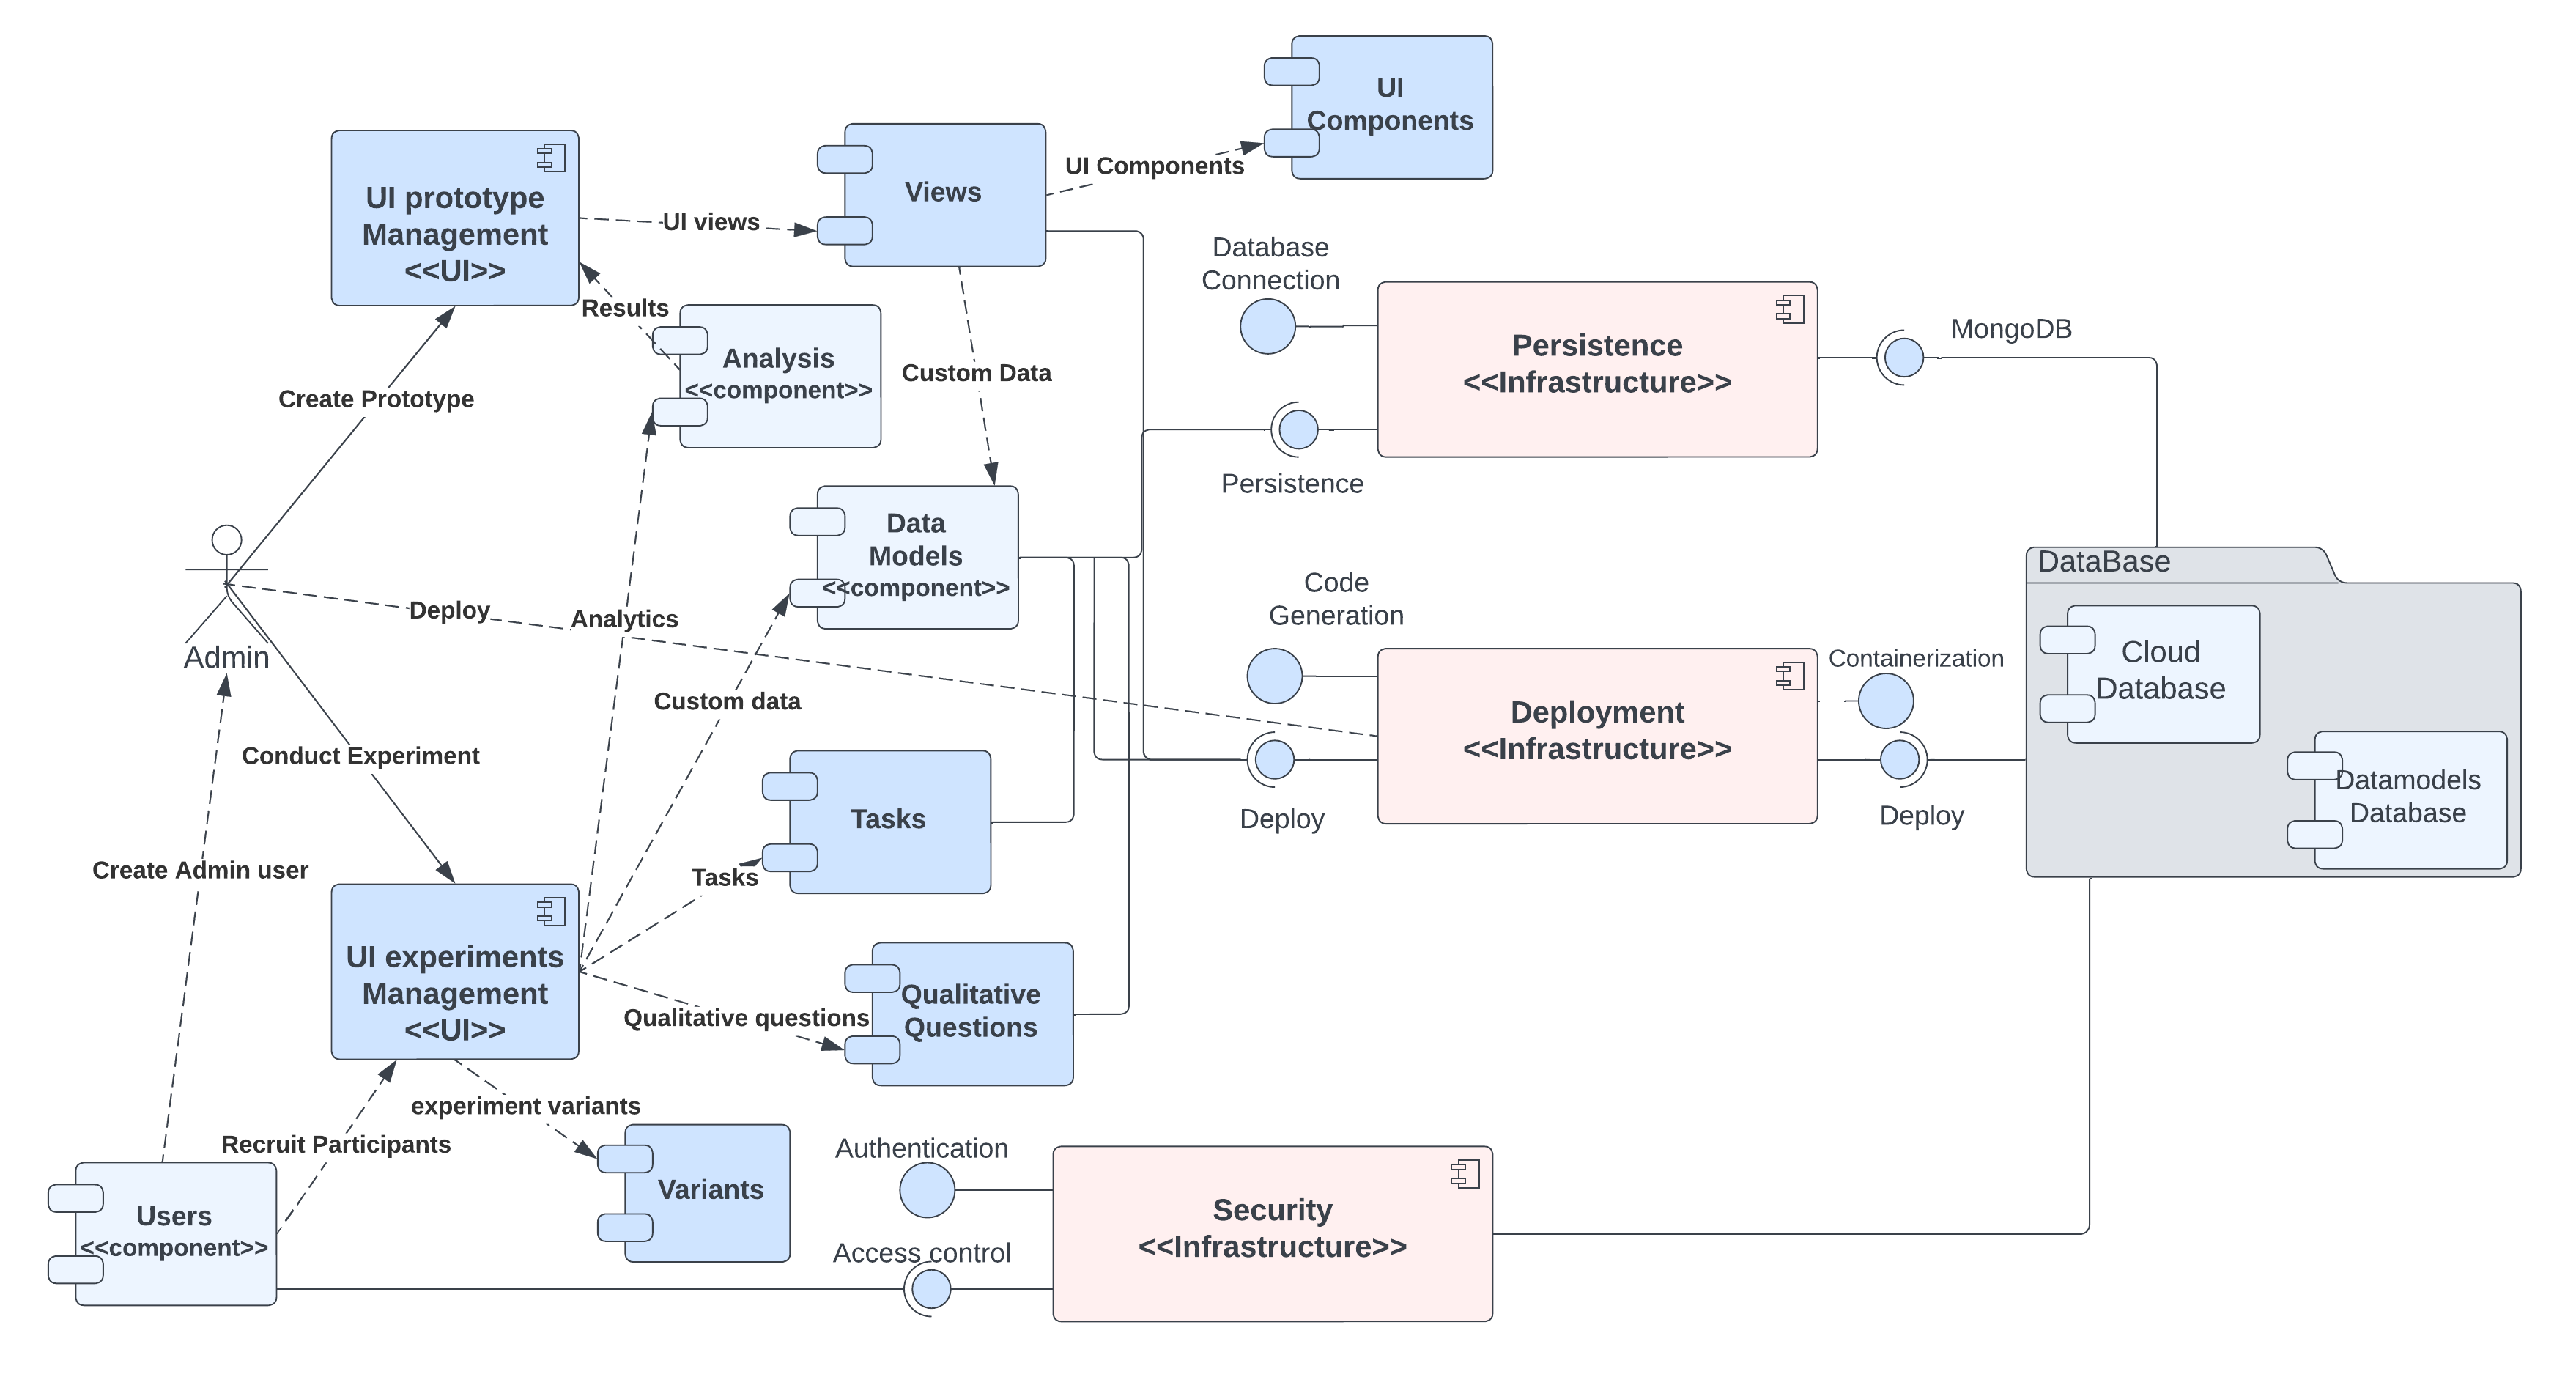
\includegraphics[width=1.1\textwidth]{Component_Diagram.png} 
    \caption[Component Diagram]{Component Diagram of our UI Prototyping tool}
    \label{fig:sc:componentD}
\end{figure}
The component diagram shows the different modules and components of the UI prototyping tool and how they interact with each other during the execution of the tool.
To better understand our component diagram, we explain with the help of a Movie streaming software\footnote{Similar to the famous movie streaming services.}.

As shown in figure (\ref{fig:sc:componentD}), the \textit{Users Component} is first used to create an \textit{Admin} user. 
Next, you create a UI prototype using the UI prototype Management with that admin user. 
This component represents the prototyping tool's UI consisting of different screens in a Views component. 
Each screen can contain UI elements (e.g., Buttons, TextBox, Input, etc.) used to navigate different screens.
From our movies example, we create different views like HomePage (which is the starting point of the application), SearchMoviesPage (used to search movies), and ViewPage (view to display various movies), and with the help of \textit{Button} \ac{ui} element navigate to various screens.
It is important to note that the \textit{Data Module component} sends custom data to the \textit{Views component} (e.g., sending different movies to screen ViewPage).
The \textit{Data Module} component is used to store and provide various custom data for displaying them on screens.
Once the UI prototype is ready, the admin user can create UI experiments using the \textit{UI Experimentation Management}.

First, we create an experiment and its different variants (e.g., \textit{ViewExperiment} as an experiment with its variants \textit{GridViewMode} and \textit{ListViewMode} displaying the movies in a grid and list view respectively). 
While creating the variants, we need to specify the percentage used to distribute the participant groups while conducting the experiment (e.g., The variant \textit{GridViewMode} with 40\% means that of the participants 40\% will be allocated to this variant and the rest to \textit{ListViewMode}).
Since our solution approach includes a task-based usability test to get user feedback, the admin user must create various tasks supported by the \textit{Tasks} component (e.g., Navigate to a movie titled ``Transformers'').
With this, we collect participants' quantitative data (like the time to complete the task, the path taken by the participant, and the number of unsuccessful attempts). 
Additionally, the admin user should add qualitative questions to collect qualitative feedback for our solution approach (e.g., ``How satisfied are you with the ease of completing this task?'').
Next, we create the participants for our experiment, which can be done using the \textit{User} component, which provides users for participation.

When the admin users have configured everything, they can start with the experimentation using the \textit{Deployment} infrastructure. 
The deployment infrastructure uses the microservice architecture to deploy all the components as they are independently built. 
The admin should deploy all the components using one button click and ask users to participate in the experiment. 
After the experiment, the admin user can get analytics using the \textit{Analysis} component. 
It provides graphical results of the quantitative analysis of different participants. 
We can also analyze the qualitative analysis using that same component and then decide on the winner variant. 
The results are then passed on to the UI prototype management component, which revises its model for the entire population.  
For the whole application, the \textit{Data Persistance} infrastructure represents the module that manages data persistence in the UI prototyping tool, and \textit{Security} infrastructure is used for access control of the participants and admin users.

\section{Persistance}
\label{sc:section:persistance}

\paragraph{Database connection}
\paragraph{Database persistance}

\section{Deployment}
\label{sc:section:deployment}

\paragraph{Code Generation}
\paragraph{Containerization}

\section{Security}
\label{sc:section:security}

\paragraph{Access control}
\paragraph{Authentication mechanisms}

\section{Experimentation management}
\label{sc:section:experimentation}

\paragraph{Creating Tasks}

\paragraph{Data Models}

\paragraph{User Management}

\paragraph{Qualitative Questions}